% How forcing is sampled from yearly to monthly
\begin{frame}[plain]{Preparing NorESM data}

    \begin{figure}
        \centering
        % \inputpgf{../figures/noresm_frc_dark.pgf}
        \includegraphics[width=\linewidth]{../figures/noresm_frc_dark.pdf}
    \end{figure}

    \note{
        Two approaches:
        \begin{enumerate}
            \item Expand forcing by repeating elements to monthly resolution (original is the dotted signal)
                \setcounter{prep_note_count}{\value{enumi}}
        \end{enumerate}
    }

\end{frame}

\begin{frame}[plain]{Preparing NorESM data}

  \begin{figure}
    \centering
    % \inputpgf{../figures/noresm_temp_dark.pgf}
    \includegraphics[width=\linewidth]{../figures/noresm_temp_dark.pdf}
  \end{figure}

  \note{
    \begin{enumerate}
    \setcounter{enumi}{\value{prep_note_count}}
  \item Or average out temperature to yearly resolution (original is the solid signal)
  \end{enumerate}
  }

\end{frame}

\begin{frame}[plain]{Re-sample response function}

  \begin{figure}
    \centering
    \tikz[baseline]{
      \node[anchor=south] (n1) {\includegraphics[width=.5\linewidth]{../figures/noresm_raw_dark.pdf}};
    }
  \end{figure}

  \vspace{-7mm}
  \begin{center}
    % {\color{MainBlue!35}\textsc{deconvolution}}
    {\pgfsetfillopacity{0.35}
      \textsc{deconvolution}
    }
    \pgfsetfillopacity{1}
  \end{center}\vspace{-3mm}

  \begin{tikzpicture}[remember picture]
    \node[align=top] (t1) {\includegraphics[width=\linewidth]{../figures/response_func_noresm_all_dark.pdf}};
  \end{tikzpicture}

  \begin{tikzpicture}[overlay]
    \path[->,white]<2> (n1) edge (2,5); %(t1.north west);
    \path[->,white]<3> (n1) edge (5.4,5); %(t1.north);
    \path[->,white]<4> (n1) edge (9,5); %(t1.north east);
  \end{tikzpicture}

  \note<+>{
  \begin{itemize}
    \item Due to re-sampling of the forcing and temperature signals, we create
      the response function in three different ways
    \item The solid green lines are the result of deconvolution using the
      NorESM dataset, with A and B coming from monthly resolved data and C from
      yearly resolved data
  \end{itemize}
  }
  \note<+>{
  \begin{itemize}
    \item In A, the response function is sampled only at whole years, starting
      at \(0, 1, 2, \ldots\)
  \end{itemize}
  }
  \note<+>{
  \begin{itemize}
    \item In B, the response function is sampled by doing a forward mean over
      twelve data points, that is, over the months in a year
    \item The value of the yearly resolved response function at year zero is
      the mean of all twelve months from the monthly resolved response function
  \end{itemize}
  }
  \note<+>{
  \begin{itemize}
    \item In C, the response function from the deconvolution already have
      yearly resolution and is only scaled by \(a_0\)
    \item We re-sample to yearly resolution since the proxy data we want to
      test against have resolution down to one year
  \end{itemize}
  }

\end{frame}

\begin{frame}[plain]{Temperature of last two millennia}

  \begin{figure}
    \centering%
    \includegraphics<1>[width=\linewidth]{../figures/estimate_historic/best_fit_raw_temps_dark.pdf}%
    \includegraphics<2>[width=\linewidth]{../figures/estimate_historic/best_fit_raw_temps2_dark.pdf}%
    \includegraphics<3>[width=\linewidth]{../figures/estimate_historic/best_fit_raw_temps3_dark.pdf}%
  \end{figure}

  \note<+>{
  \begin{itemize}
    \item We first look at how well the response function from A recreates
      historic temperature
    \item These are reconstructed temperature and forcing data sets from the
      last two millennia, with temperature in red and forcing in blue (note the
      scale is different by a factor ten)
    \item The response function we obtained is convolved with the blue forcing
      signal, and give an estimated temperature shown as the yellow line
    \item Estimated temperature largely capture the temperature from the forcing
  \end{itemize}
  }
  \note<+>{
  \begin{itemize}
    \item Using response function B yields similar results
    \item Volcanoes give smaller temperature respone using alternative B
      compared to A, othervise similar trend
  \end{itemize}
  }
  \note<+>{
  \begin{itemize}
    \item Again we see a very similar result is obtained from C, showing the
      consistency of the deconvolution algorithm
    \item How the response functions treat fast events differ, but not the trend
  \end{itemize}
  }

\end{frame}

\begin{frame}[plain]{Temperature of \(4\times\ce{CO2}\) experiment}

  \begin{figure}
    \centering
    % 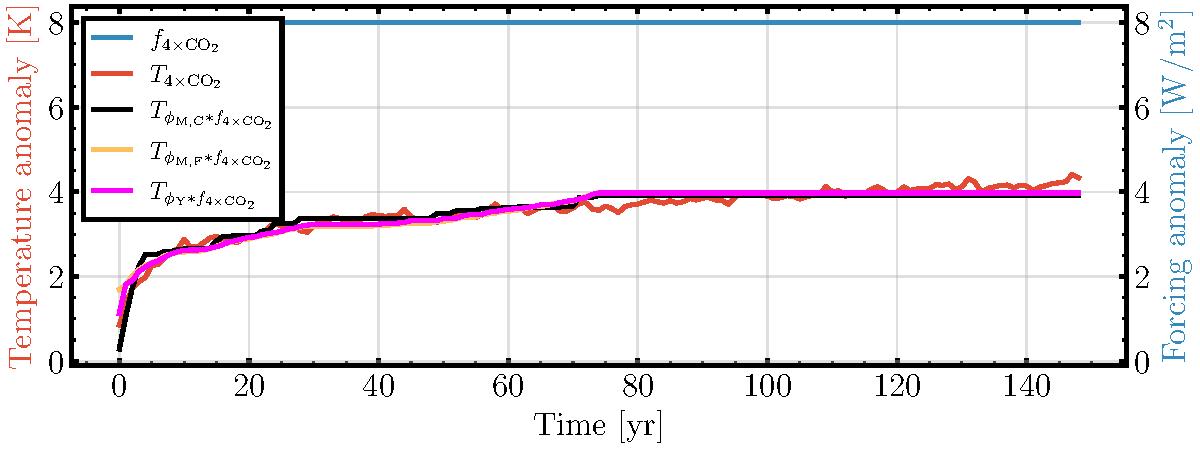
\includegraphics[width=\linewidth]{../figures/estimate_historic/all_temp_abrupt.pdf}%
    \includegraphics<1>[width=\linewidth]{../figures/estimate_historic/temp_abrupt1_dark.pdf}%
    \includegraphics<2>[width=\linewidth]{../figures/estimate_historic/temp_abrupt2_dark.pdf}%
    \includegraphics<3>[width=\linewidth]{../figures/estimate_historic/temp_abrupt3_dark.pdf}%
  \end{figure}

  \note<+>{
  \begin{itemize}
    \item Taking a look back at the climate sensitivity, we now convolve the
      three response functions with a constant forcing representing a
      quadrupling of \ce{CO2} concentration from pre-industrial levels
    \item This is a common experiment to do to decide equilibrium climate
      sensitivity, where the temperature at two different equilibria is
      compared
    \item Able to capture the shape of a NorESM \(4\times\ce{CO2}\) experiment
  \end{itemize}
  }
  \note<+>{
  \begin{itemize}
    \item Compared to a it differ in the first year, but again the response
      function give a temperature estimate that follow the shape of the
      temperature from simulation
  \end{itemize}
  }
  \note<+>{
  \begin{itemize}
    \item Same can be found when using C, first year differ between the three
      versions, but they all capture the trend
  \end{itemize}
  }

\end{frame}

% \subsection{Power spectra}

\begin{frame}[plain]{Power spectra}

  \begin{figure}
    \centering
    \includegraphics[width=\linewidth]{../figures/estimate_historic/all_psd_dark.pdf}
  \end{figure}

  \note<+>{
  \begin{itemize}
    \item The residuals from the estimated historical temperature should have
      same statistics as a simulation without forcing (only noise / internal
      variability)
    \item Good agreement between control run and residuals
  \end{itemize}
  }

\end{frame}
